\section{Abbildungen: $\mathbb{R} \rightarrow \mathbb{R}^n$}

\subsection{Linearisierung}
$f(t+\Delta t) \approx f(t) + \Delta t \cdot f'(t)$

\subsubsection{Bogenlänge}
\begin{itemize}
	\item Normale Funktionen: $L_{a,b} \approx \int_a^b \sqrt{1+f'(x)^2} dx$
	\item Parametrisiert: \\
	\begin{displaymath}
		f: x \rightarrow
		\begin{pmatrix}
			f_1(x) \\ f_2(x) \\ f_3(x)
		\end{pmatrix}
		\Rightarrow
		L_{a,b} = \int_a^b \bigg |
		\begin{pmatrix}
			f_1'(x) \\ f_2'(x) \\ f_3'(x)
		\end{pmatrix}
		\bigg |_2 dx
	\end{displaymath}
\end{itemize}

\subsubsection{Krümmung}
\begin{itemize}
	\item $K(x) = \frac{f''(x)}{\sqrt{1+f'(x)^2}^3}$
	\item Krümmungskreis Radius: $\frac{1}{K(x)}$ \\
	\begin{figure}[h!]
		\centering
		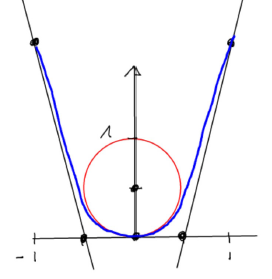
\includegraphics[scale=.5]{pics/kruemmungskreis}
		\caption{Krümmunkskreis im Scheitelpunkt}
	\end{figure}
\end{itemize}
